\section*{Concept}
\addcontentsline{toc}{section}{Concept}
\subsection*{From Idea to Mockup}

Goal of this concept is to visualize the phenomena of a heating process inside a furnace. The development process began by discussing the main parts of the task description and by researching about existing systems in this field. At first, a standard \ac{SCADA} system was thought to be the goal of the concept. With the design principles described by Zuehlke \cite{Zhlke2012NutzergerechteEV} and the ISO-Standard 9241 \cite{din_9241-110} in mind a wireframe was made.

This first step was very important because learning, how to structure the \ac{SCADA} system, is vital. Additional insights from illustrations and theoretical foundations for the design process, were given by Jamieson \cite{Jamieson2001} and Vicente \cite{Vicente1992}. As learned from the \ac{MMST}-lecture, all project team members got a specific role within the user-centered design process. That way the theoretical groundwork and the team building measurements for the project were finished.

It was clear that interaction with the visualization system has to be as simple as possible and the decision was made to go for a one page all access solution. With a one page solution the user cannot be distracted from the process and always has it in clear sight. In case of an alarm message as shown in the appendix figure \ref{fig:appendix_error}, the operator can quickly react and does not have to switch between pages of the \ac{UI}. Furthermore, the \ac{UI} had to be divided into major sections like header, content section, and footer. Thus, a high level of content related grouping has been achieved, which the user is already familiar with from everyday interfaces. Together with the information from the task description all parts were designed with regard to consistency, cohesion and proximity. The content section was further divided into the visualization of the furnace itself, a control block for the three input streams and a process summary, which was thought to show a graph of the process. 

Soon after the initial wireframe, the "\ac{SCADA}-like" system was concretized and the decision was made to display it on a Full HD\footnote{Full HD = 16:9 aspect ratio with a resolution of 1920x1080 pixels} monitor. Like data from StatCounter Global Stats \cite{statcounterResolution} recently showed, Full-HD is used by 25.7 percent of users in the United Kingdom. That way the best text readability and user friendly monitor resolution for the system proposed is achieved. That resulted in turning the existing wireframe (figure \ref{fig:Wireframes}) into a detailed mockup (figure \ref{fig:FigmaMockup}) with correct aspect ratios.

\begin{figure*}[ht]
    \centering
    \begin{subfigure}{0.5\textwidth}
        \centering
        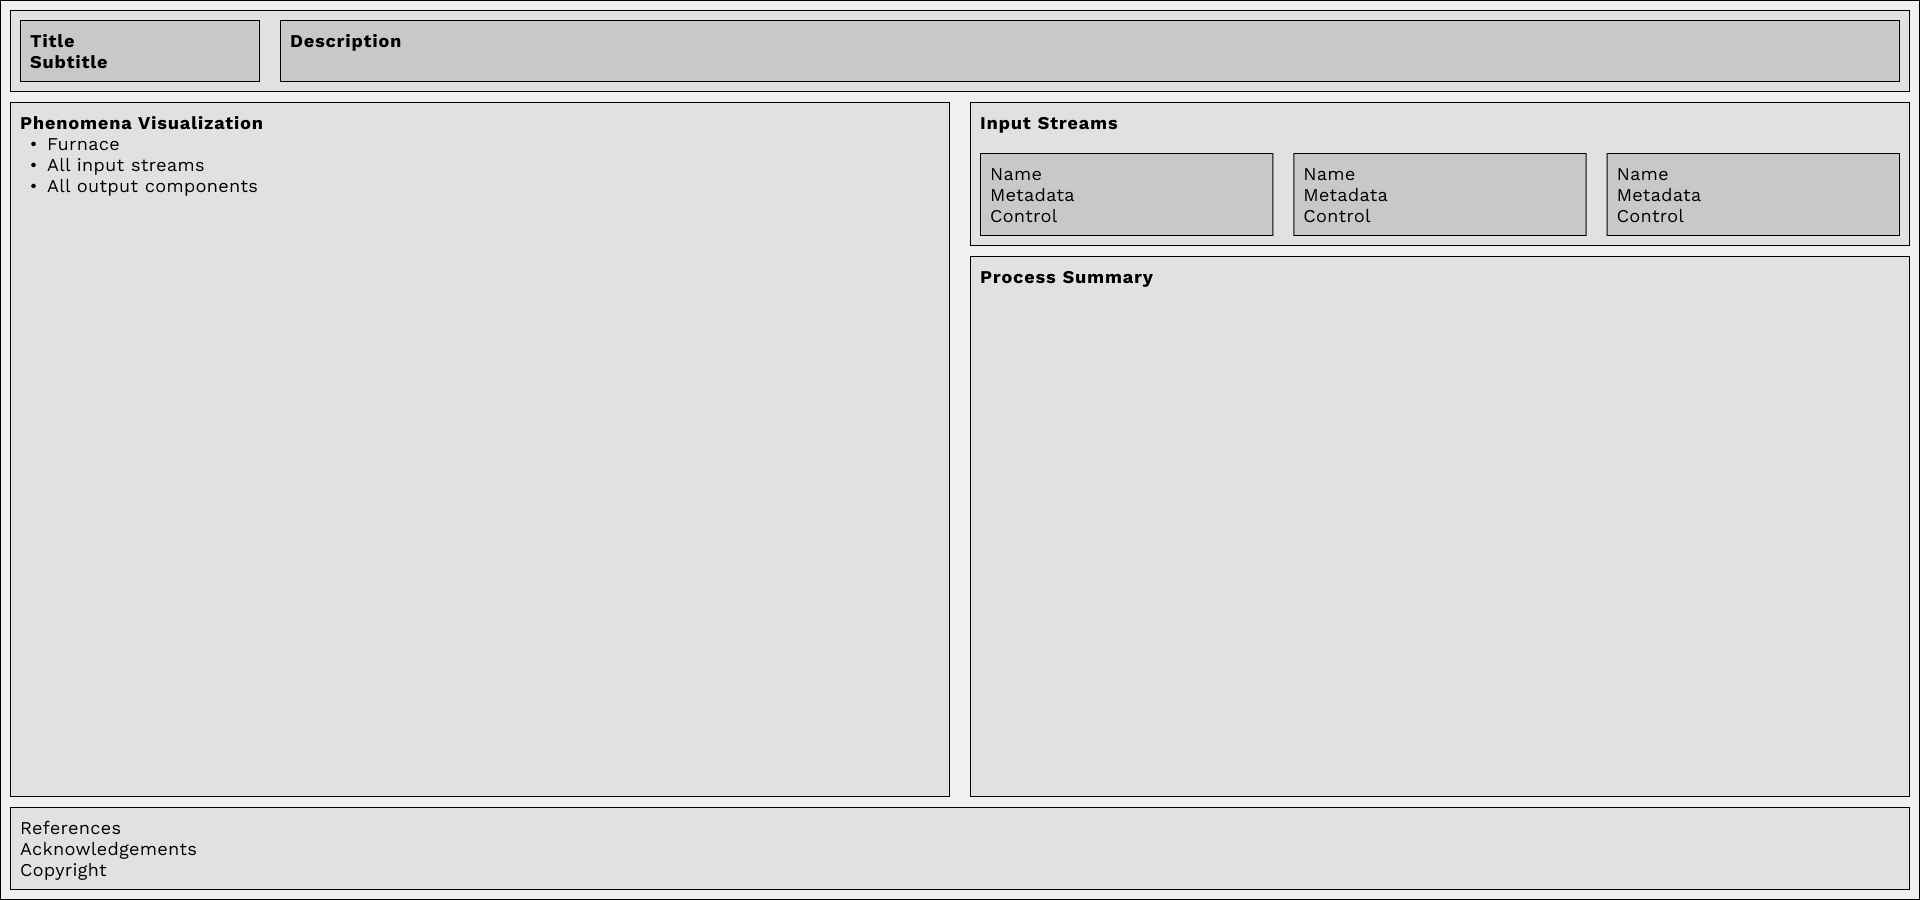
\includegraphics[width=0.9\linewidth]{images/concept/wireframes/Wireframe_1_figma.png}
        \caption{}
    \end{subfigure}%
    \begin{subfigure}{0.5\textwidth}
        \centering
        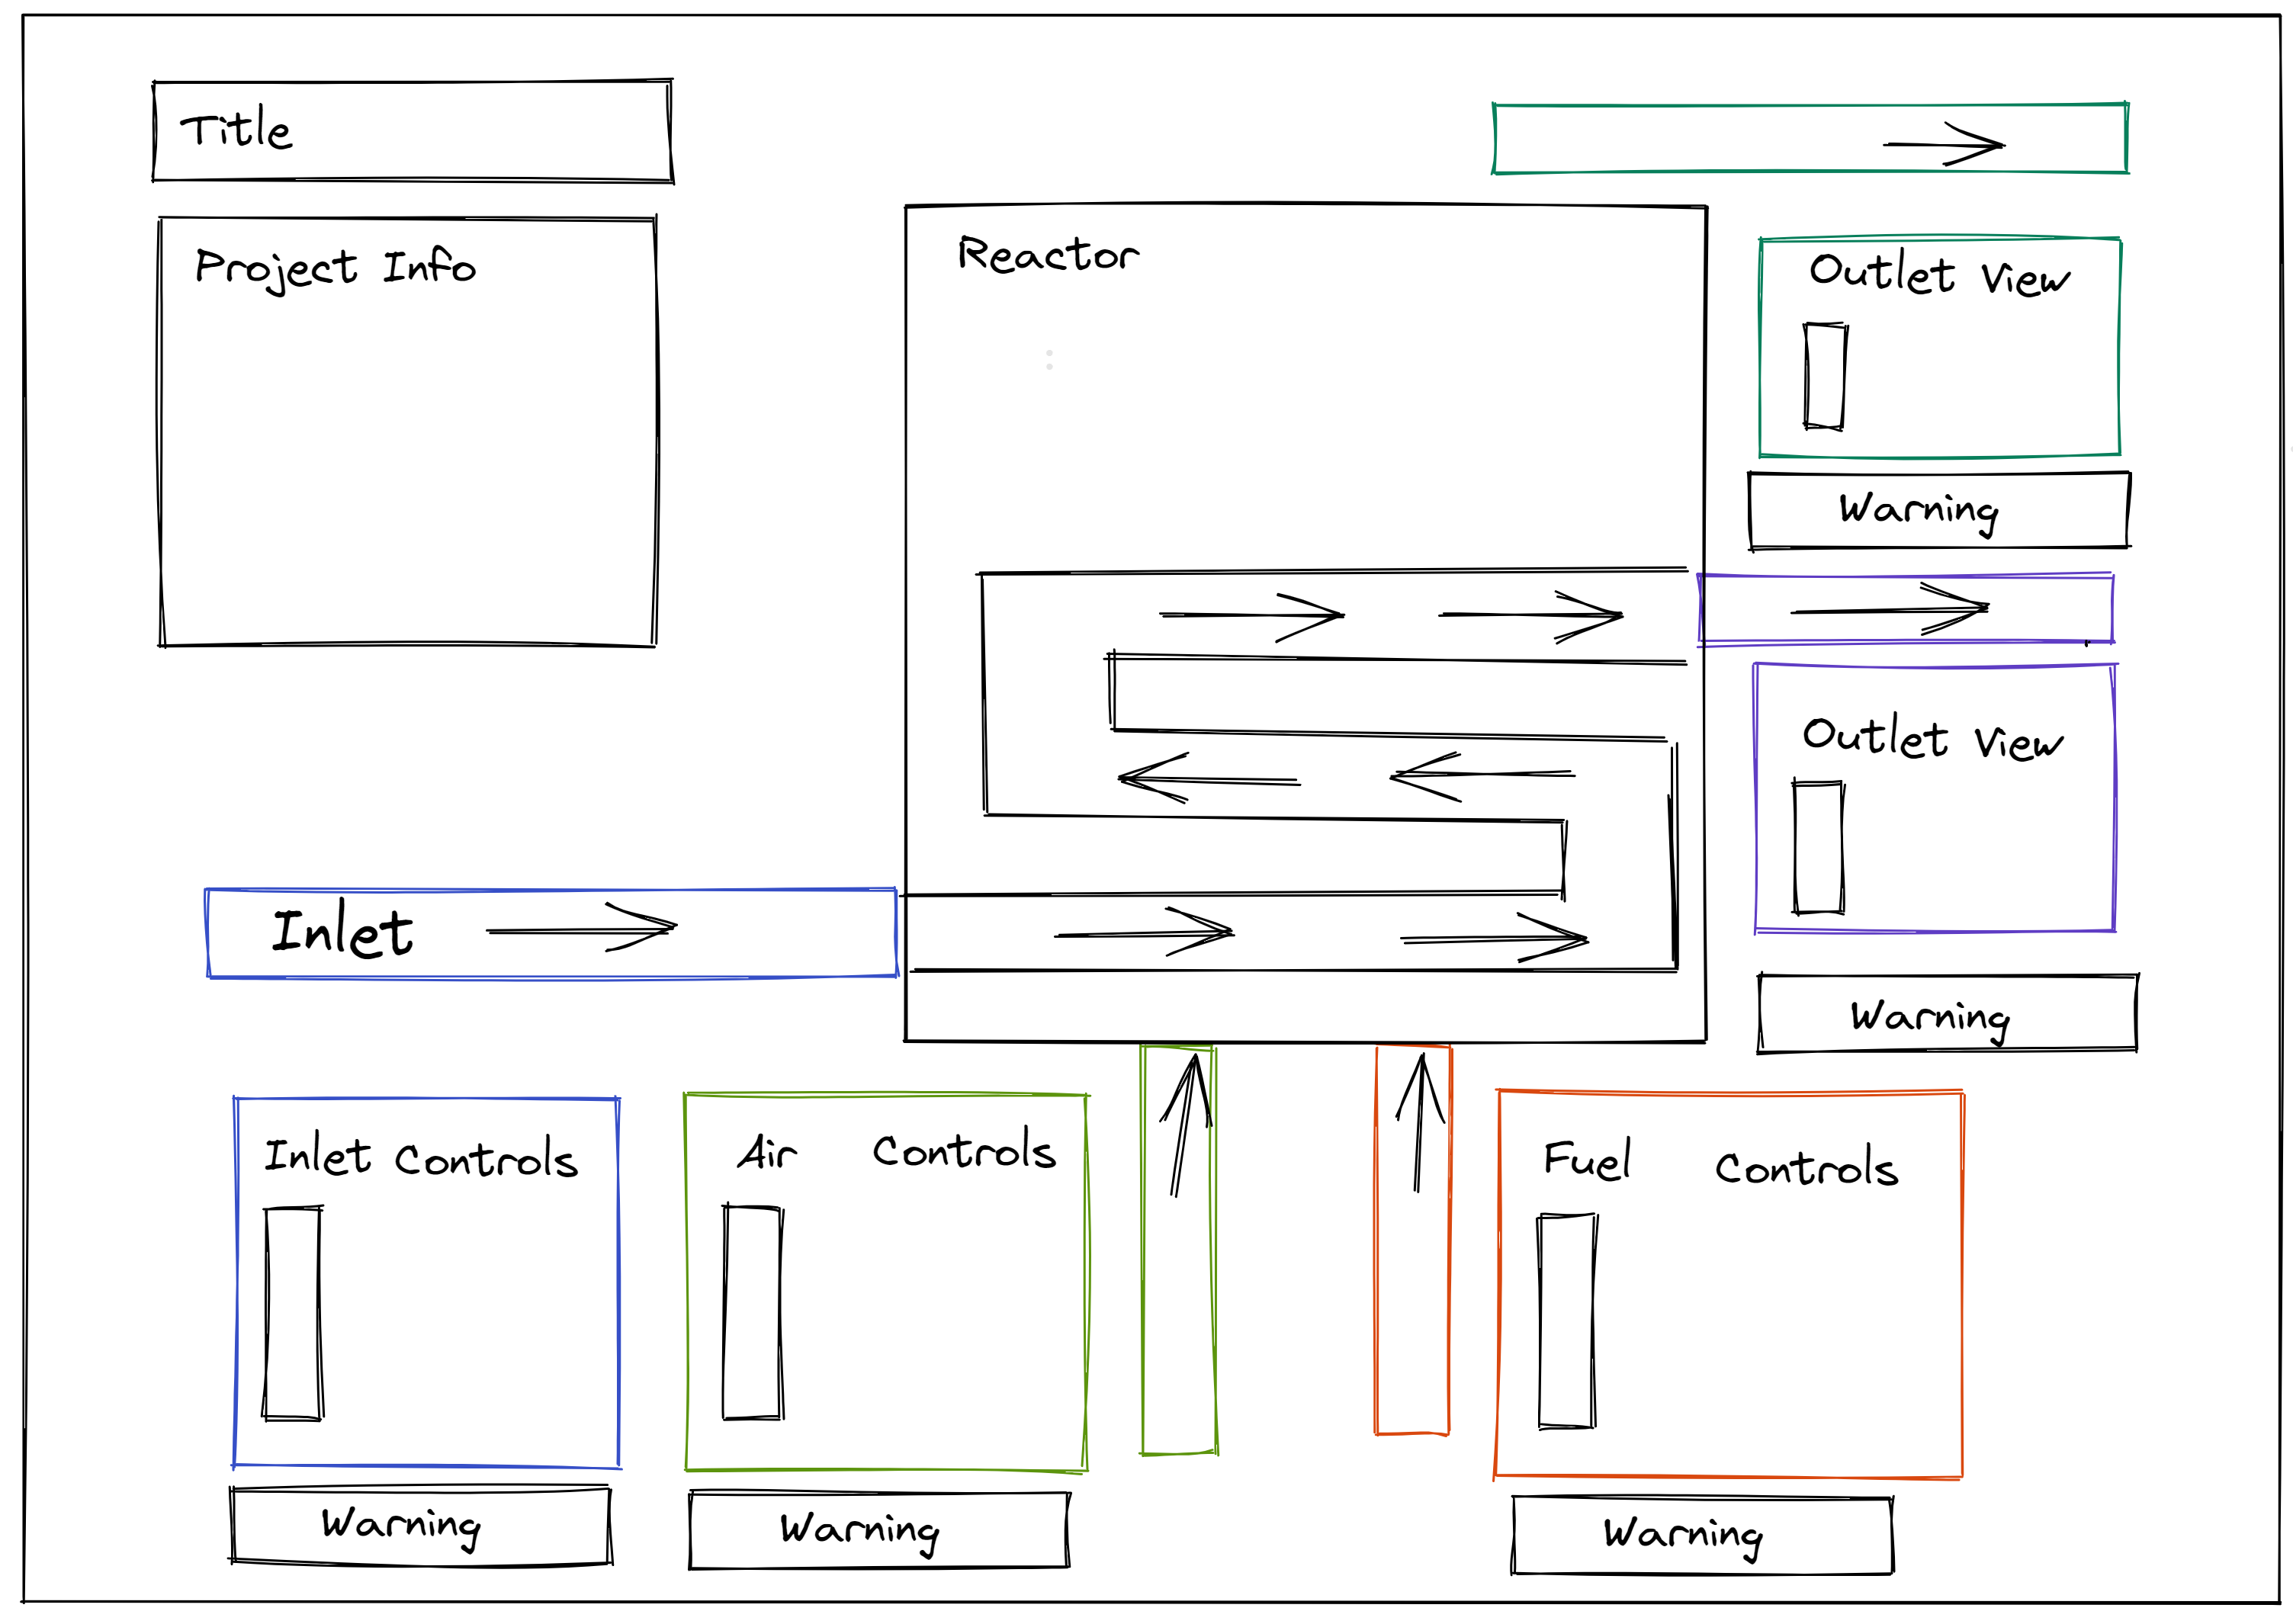
\includegraphics[width=0.7\linewidth]{images/concept/wireframes/Wireframe_2_axure.png}
        \caption{}
    \end{subfigure}
    \caption { (a) figma wireframe (b) axure wireframe}
\label{fig:Wireframes}
\end{figure*}

\begin{figure}[ht]
    \centering
    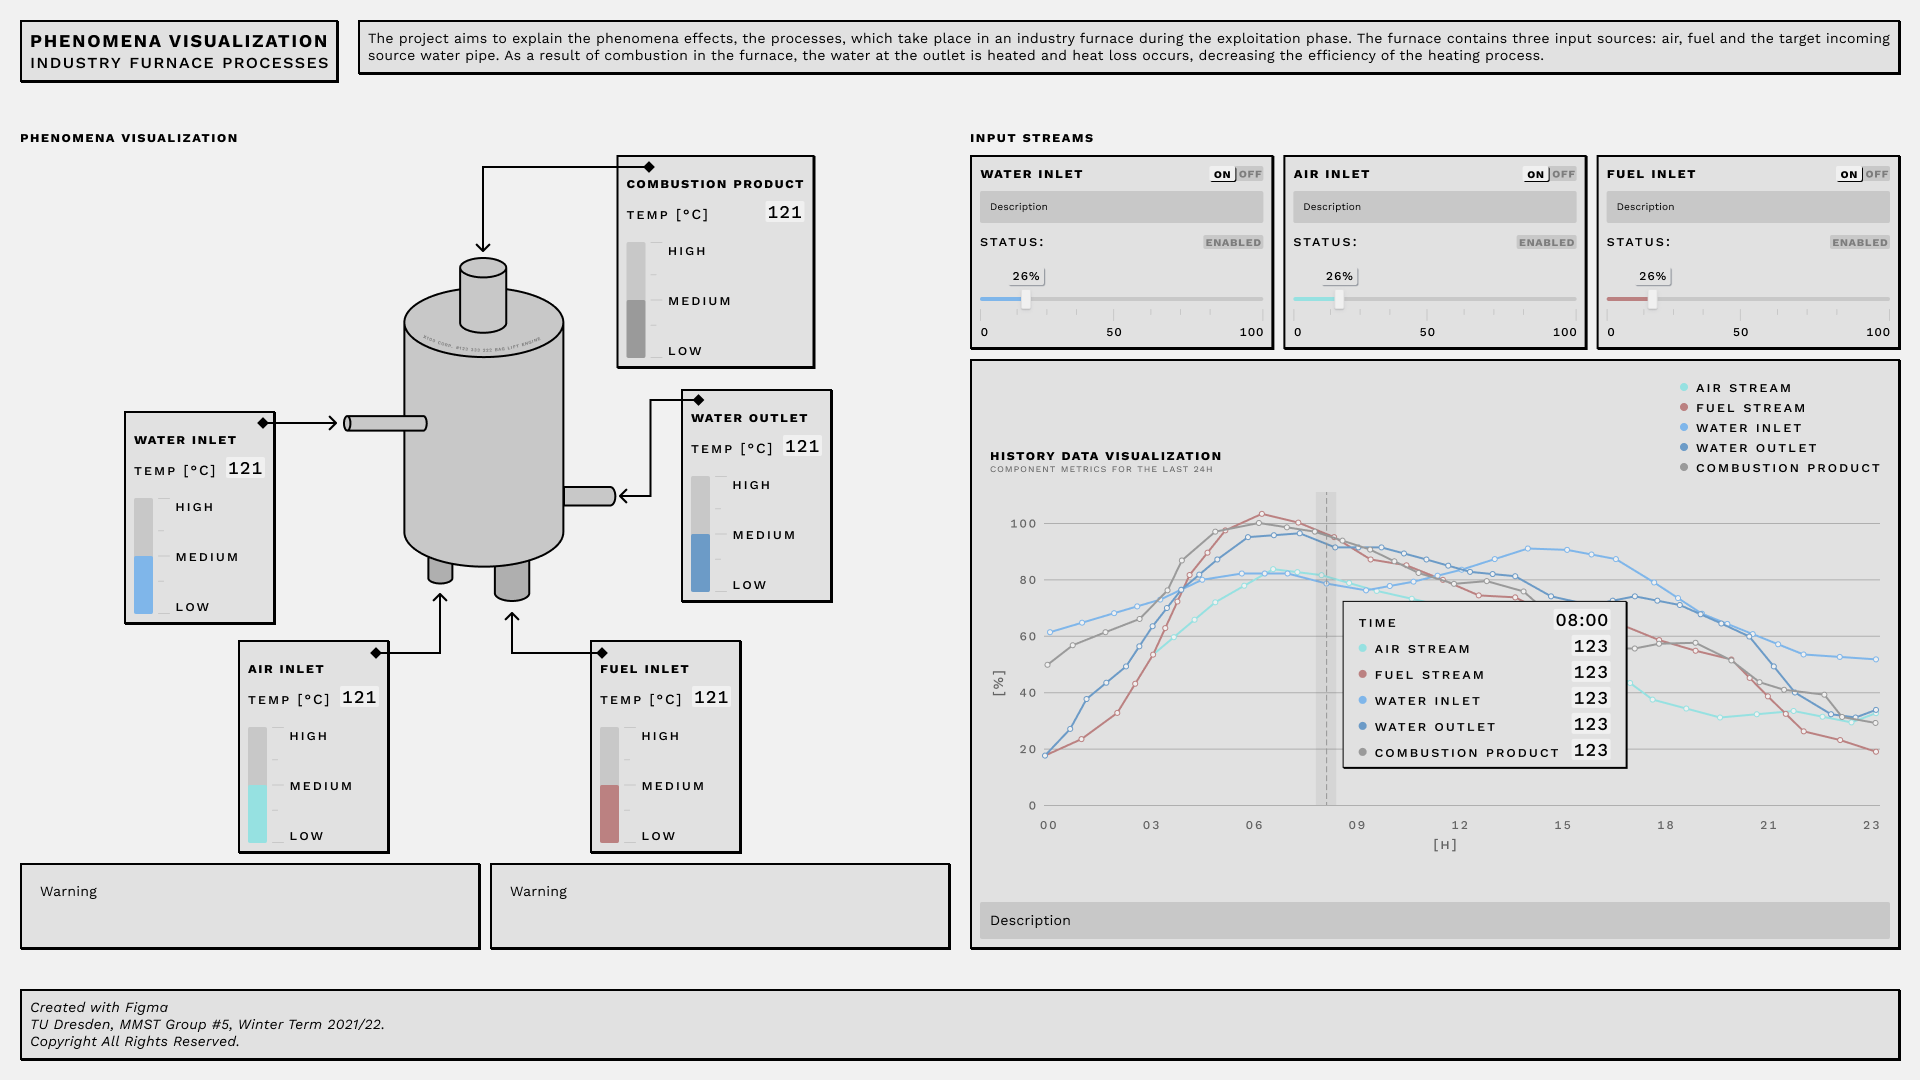
\includegraphics[width=0.6\linewidth]{images/concept/mockup/mockup_v1_figma.png}
    \caption{figma mockup}
    \label{fig:FigmaMockup}
\end{figure}

Both, wireframe and mockup were made in Figma\footnote{Figma Website: https://www.figma.com/}, but in the end Axure\footnote{Axure Website: https://www.axure.com/} had to be used to build the prototype. Additionally, after reviewing the Figma wireframe and mockup, it was clear that the visualization of the phenomena happening inside the furnace are not represented enough. Therefore, the Figma design had to be changed significantly. Ultimately, the resulting prototype should be nothing like a standard industrial \ac{SCADA} system. This resulted in a redo of the design process. With this new approach to the design and insights from the first wireframe, a new concept shown in Figure \ref{fig:Wireframes} was developed.

The heating process in the furnace and its visualization is the major part of the design and should be displayed in the center of the screen. As learned from the \ac{MMST}-lecture and mentioned by Zuehlke\cite{Zhlke2012NutzergerechteEV} and Jenkins et al. \cite{Jenkins2013}, there are certain laws and design principles which have to be kept in mind when designing an interface. These design principles include cohesion, proximity and clearness of the interface elements. The need for clarity, symmetry and order is embedded in a humans perception. Therefore every element of the system had to be well aligned and situated within the screen area following these principles. As a result, a first mockup was developed in Axure. As further alterations to the mockup were made, the animation of the different elements got into focus, which ultimately led to a straight horizontal pipe design instead of using a winded pipe design, like displayed in Figure \ref{fig:axurewiremockup}.

   
\begin{figure}[ht]
    \centering
    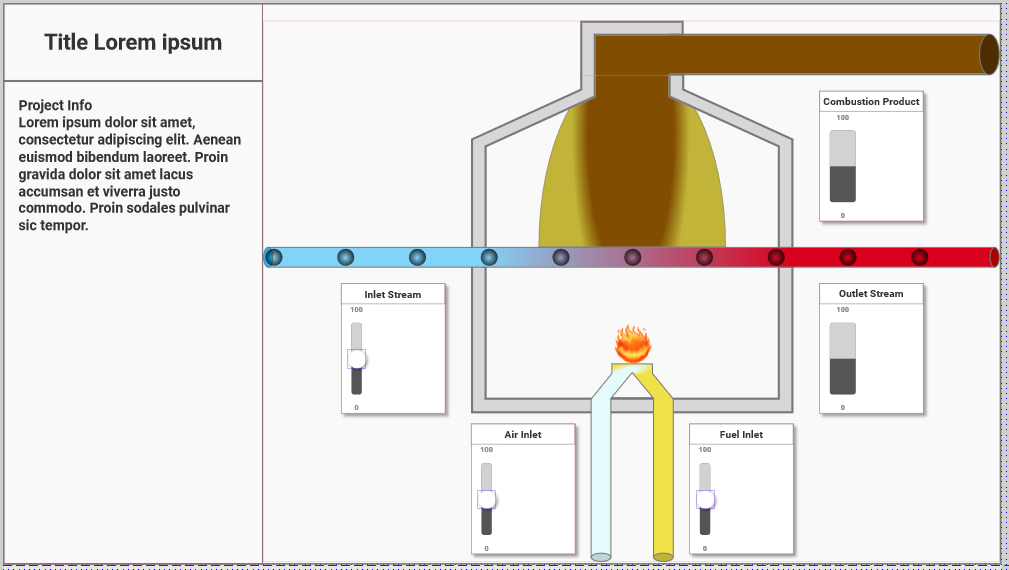
\includegraphics[width=0.6\linewidth]{images/concept/mockup/mockup_v3_axure.png}
    \caption{axure mockup}
    \label{fig:axurewiremockup}
\end{figure}

\subsection*{Visualization of the Major Elements}

The design consists of seven major elements which had to be conceptualized in a user friendly and easy to understand fashion. These elements are described further in this section. Pictures of every element and the development process can be found in the appendix.

\begin{enumerate}
  \item The ON/OFF switch on the top left corner acts as a clear indicator of the system status. Both text("ON","OFF") and color("green","red") were used to consolidate the status. See appendix, figure \ref{fig:appendix_heat_loss_systempower} (a)
  \item The feed flow moves through the furnace at a user defined rate and is thus influencing the feed volume and temperature. See appendix, figure \ref{fig:appendix_flow_pipe}
  \item The feed flow changes its color in relation to the temperature within the furnace. The feed temperature is displayed by using a cold color such as blue symbolizing a cold feed and red as a warm color symbolizing a warm feed. This way, the user can easily distinguish between a warm and cold feed. Furthermore, the temperature of the outlet is displayed by the status indicator on the right hand side of the furnace as well. The colors of the outlet graph are consistent to the colors used for the feed. See appendix, figure \ref{fig:appendix_flow_pipe} and \ref{fig:feed_output}
  \item Fuel and air are mixed and ignited inside the combustion chamber of the furnace and a flame changes its size depending on the amount of air and fuel flowing into the furnace. The size of the flame and the corrugated arrows inside the furnace showcase the amount of heat. By using a change in size a sense of intensity is created. See appendix, figure \ref{fig:appendix_combustion_reaction}
  \item The heat loss of the furnace is displayed by a corrugated arrow on the left flat side of the furnace lid. As shown by Jenkins et al.  \cite{Jenkins2013} corrugated arrows are advantageous for displaying heat transfer inside the furnace. The arrow will change its size depending on the size of the fire. Additionally the heat transfer is shown by a reduced amount of arrows above the feed pipe.  See appendix, figure \ref{fig:appendix_heat_loss_systempower} (b)
  \item The brightness of the combustion product is altered depending on the size of the combustion process. This element is shown on the top right of the furnace and serves as an indicator for the amount of combustion products exiting the furnace. A light grey indicates a small combustion and a dark grey indicates a large combustion. See appendix, figure \ref{fig:appendix_combustion_product}
  \item Potentially hazardous and dangerous situations are displayed by error warnings. In addition to a red error warning on the left-hand side of the \ac{UI} a flashing error symbol next to the control element which has to be altered to leave the dangerous situation was created.  See appendix, figure \ref{fig:appendix_error}
\end{enumerate}

\subsection*{Interactive elements and dynamic behavior of the prototype}

The \ac{UX} elements were designed following the seven interaction principles, mentioned in the \ac{MMST}-lecture. These interaction principles are defined in DIN EN ISO 9241-110 \cite{din_9241-110}. The four components the user can interact with are the power button to en- and disable the whole system and three sliders to control the inputs of the furnace. This keeps it consistent with the control-elements of the real furnace and therefore stays conform to expectations. The operator knows of the correlations between the controls of the phenomena visualization and the furnace control. This increases the learnability as well as the robustness against user errors, as the user of the visualization is a furnace operator with knowledge about the control parameters. 

The fuel, air and feed flow can be controlled continuously through valves or other flow limiters. Sliders have been chosen to enable a continuous alteration of the three input flows. The vertical display of parameters is interpreted as a representation for a min-max-scale by most people, as they are found in many everyday applications reaching from measuring cups to thermometers. Therefore, the sliders are placed vertically and allow for a limitation of the flow from 0\% to 100\%.

To raise user engagement, the visual representation of the system behavior needs to be appealing and easy to understand. The prototype should display the system parameters as efficient as possible while also giving clear indications about changes. As described in the requirements section, there is a variety of information that needs to be conveyed to the user. When the combustion increases or the feed flow decreases, the temperature of the feed flow rises and vice versa. This will be displayed by a continuous change in color from light blue to dark red. This visualization entails the risk of the user assuming that a high outlet temperature is the desired behavior of the furnace. The efficiency of a plant is defined by the percentage of energy transferred into the feed stream. The amount of energy stored in the outlet stream is proportional to the temperature multiplied by the throughput. To display this information as well, a small diagram has been placed near the outlet.

When the amount of fuel running into the furnace rises, a higher combustion takes place which is shown by a larger fire animation. As the combustion process generates more heat, the heat loss grows. To indicate that, the arrows visualizing the heat flow will enlarge and the exhaust pipe changes to a darker grey to display the increase in exhaust. The meaning of this change in color should be self-explanatory, as this is analogous to chimneys and other exhausts. At the end of the project, these assumptions about intuitiveness have to be evaluated.



